\documentclass{beamer}
\mode<presentation>
\usetheme{Boadilla}

\usepackage{amsmath,amssymb}
\usepackage{graphicx}
\usepackage{gvv}
\usepackage{listings}
\usepackage{xcolor}

% Code style
\lstset{
  basicstyle=\ttfamily\scriptsize,
  breaklines=true,
  frame=single,
  numbers=left,
  numberstyle=\tiny,
  keywordstyle=\color{blue},
  commentstyle=\color{green!50!black},
  stringstyle=\color{red!60!black},
  showstringspaces=false
}

\title{Matrix 2.6.24}
\author{ai25btech11015 -- M Sai Rithik}
\date{}

\begin{document}
\maketitle

\begin{frame}
\frametitle{Question}
Find the area of the parallelogram formed by the vectors
\[
\Vec{a} = 3\hat{i} + \hat{j} + 4\hat{k}, \qquad
\Vec{b} = \hat{i} - \hat{j} + \hat{k}.
\]
Use the cross product definition.
\end{frame}

\begin{frame}
\frametitle{Cross Product Definition}
\begin{itemize}
\item Let
\begin{align}
\Vec{A} &= \myvec{a_1 \\ a_2 \\ a_3}, \\
\Vec{B} &= \myvec{b_1 \\ b_2 \\ b_3}.
\end{align}

\item Define sub-vectors
\begin{align}
\Vec{A}_{ij} = \myvec{a_i \\ a_j}, \quad
\Vec{B}_{ij} = \myvec{b_i \\ b_j}.
\end{align}

\item The cross product is
\begin{align}
\Vec{A}\times\Vec{B} =
\myvec{
  \mydet{\Vec{A}_{23} & \Vec{B}_{23}} \\
  \mydet{\Vec{A}_{31} & \Vec{B}_{31}} \\
  \mydet{\Vec{A}_{12} & \Vec{B}_{12}}
}.
\end{align}
\end{itemize}
\end{frame}

\begin{frame}
\frametitle{Applying the Formula}
\begin{itemize}
\item For the given vectors
\begin{align}
\Vec{a} = \myvec{3 \\ 1 \\ 4}, \qquad
\Vec{b} = \myvec{1 \\ -1 \\ 1}.
\end{align}

\item Substituting:
\begin{align}
\Vec{a}\times\Vec{b} &=
\myvec{
\mydet{\myvec{1 \\ 4} & \myvec{-1 \\ 1}} \\
\mydet{\myvec{4 \\ 3} & \myvec{1 \\ 1}} \\
\mydet{\myvec{3 \\ 1} & \myvec{1 \\ -1}}
}.
\end{align}
\end{itemize}
\end{frame}

\begin{frame}
\frametitle{Simplification}
\begin{align}
\Vec{a}\times\Vec{b} &=
\myvec{
(1)(1) - (4)(-1) \\
(4)(1) - (3)(1) \\
(3)(-1) - (1)(1)
} \\
&= \myvec{5 \\ 1 \\ -4}.
\end{align}
\end{frame}

\begin{frame}
\frametitle{Area of Parallelogram}
\begin{align}
\text{Area} &= \|\Vec{a}\times\Vec{b}\| \\
&= \sqrt{5^2 + 1^2 + (-4)^2} \\
&= \sqrt{42}.
\end{align}

\[
\boxed{\text{Area} = \sqrt{42}}
\]
\end{frame}

\begin{frame}
\frametitle{Figure}
\centering
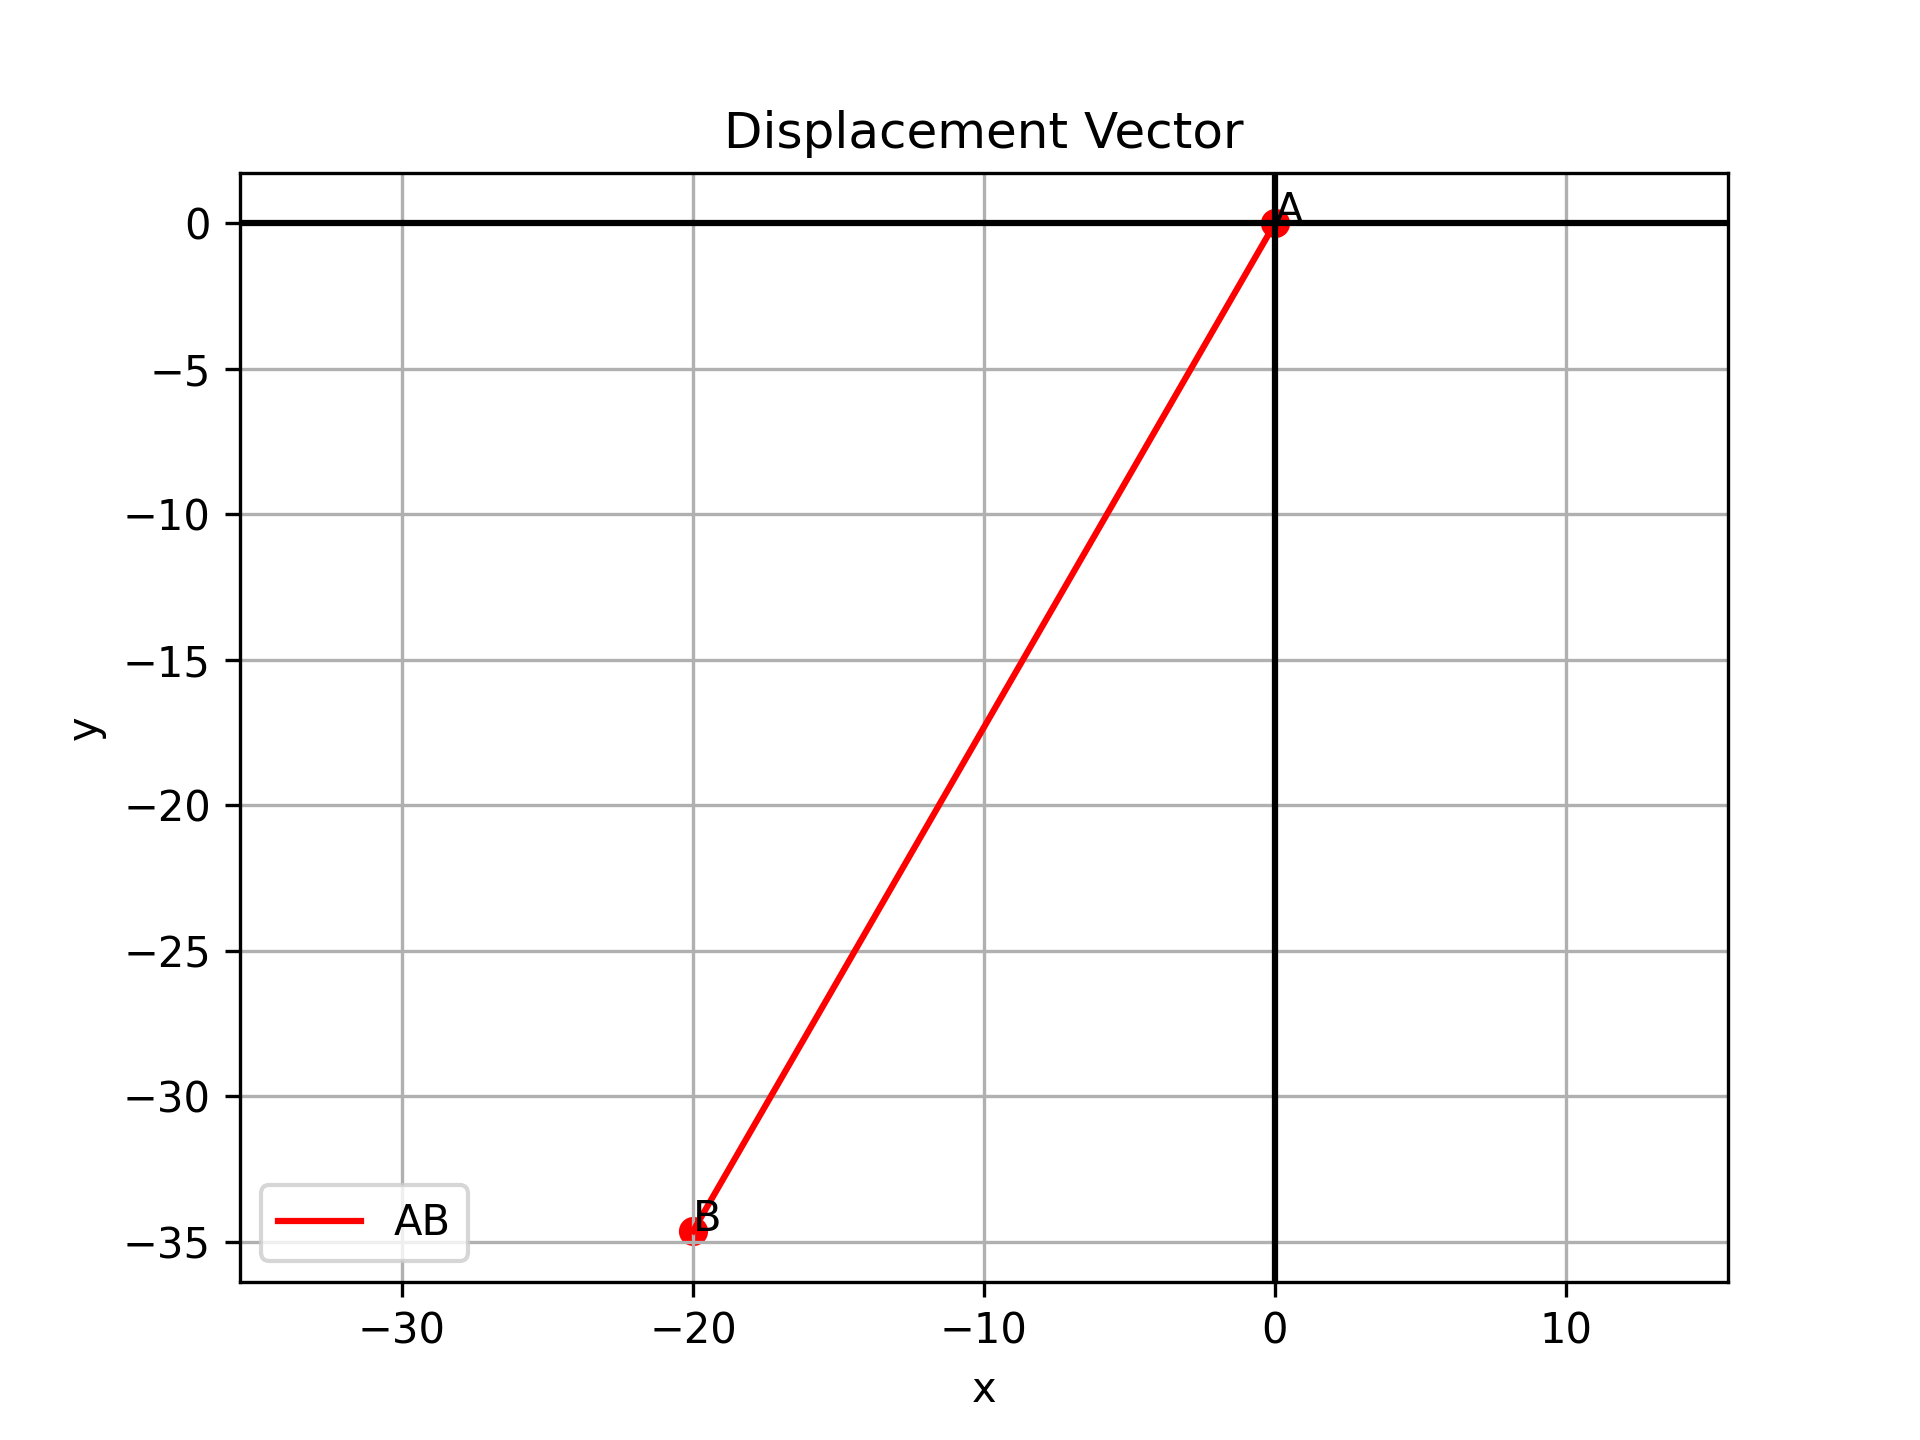
\includegraphics[width=0.6\linewidth]{figs/fig.png}
\caption{Parallelogram spanned by $\Vec{a}$ and $\Vec{b}$.}
\end{frame}

\begin{frame}[fragile]
    \frametitle{C Code}
    \begin{lstlisting}[language=C]
// C code to calculate area of parallelogram
#include <stdio.h>
#include "libs/matfun.h"
#include <math.h>

double main() {
    // create a b vectros 
    double **a = createMat(3,1);
    a[0][0] = 3;
    a[1][0] = 1;
    a[2][0] = 4;

    double **b = createMat(3,1);
    b[0][0] = 1;
    b[1][0] = -1;
    b[2][0] = 1;


    double **a_cross_b = createMat(3,1);
    a_cross_b[0][0] = a[1][0] * b[2][0] - a[2][0] * b[1][0];
    a_cross_b[1][0] = a[2][0] * b[0][0] - a[0][0] * b[2][0];
    a_cross_b[2][0] = a[0][0] * b[1][0] - a[1][0] * b[0][0];

    double area = sqrt(Matdot(a_cross_b, a_cross_b, 3));
\end{lstlisting}
\end{frame}


\begin{frame}[fragile]
    \frametitle{C Code}
    \begin{lstlisting}[language=C]
    printf("Area of the parallelogram: %lf\n", area);

    FILE *fp = fopen("var.dat", "w");
    if (fp != NULL) {
        fprintf(fp, "%lf\n", area);
        fclose(fp);
    } else {
        printf("Error opening file for writing.\n");
    }
    return area;
}
\end{lstlisting}
\end{frame}
    
\begin{frame}[fragile]
    \frametitle{Python Code}
    \begin{lstlisting}[language=Python]
import numpy as np 
from mpl_toolkits.mplot3d import Axes3D
from mpl_toolkits.mplot3d.art3d import Poly3DCollection
import ctypes
import matplotlib.pyplot as plt

# Load the shared object file
main_lib = ctypes.CDLL('./main.so')

# Define input and return types for the C function
# main_lib.main.argtypes = []
main_lib.main.restype = ctypes.c_double

# Call the C function to calculate the area
area_value = main_lib.main()
print(area_value)


with open('var.dat', 'r') as f:
	area = f.read().strip()

a = np.array([3, 1, 4])
b = np.array([1, -1, 1])
O = np.array([0, 0, 0])
\end{lstlisting}
\end{frame}

\begin{frame}[fragile]
    \frametitle{Python Code}
    \begin{lstlisting}[language=Python]
fig = plt.figure()
ax = fig.add_subplot(111, projection='3d')

# Plot vectors OA and OB
ax.quiver(*O, *a, color='r', label='OA')
ax.quiver(*O, *b, color='b', label='OB')
ax.text(a[0], a[1], a[2], 'OA', color='r', fontsize=12)
ax.text(b[0], b[1], b[2], 'OB', color='b', fontsize=12)

verts = [ [O, a, a+b, b] ]
ax.add_collection3d(Poly3DCollection(verts, alpha=0.3, facecolor='green'))

# Set limits and labels
ax.set_xlim([0, max(a[0], b[0], a[0]+b[0])+1])
ax.set_ylim([min(0, a[1], b[1], a[1]+b[1])-1, max(a[1], b[1], a[1]+b[1])+1])
ax.set_zlim([0, max(a[2], b[2], a[2]+b[2])+1])
ax.set_xlabel('X')
ax.set_ylabel('Y')
ax.set_zlabel('Z')
ax.legend()


\end{lstlisting}
\end{frame}




\begin{frame}[fragile]
    \frametitle{Python Code}
    \begin{lstlisting}[language=Python]
plt.tight_layout()
plt.savefig('../figs/fig.png')
plt.close()
\end{lstlisting}
\end{frame}
\end{document}
